\documentclass[margin,line]{resume}

\definecolor{sidebarcolor}{HTML}{FC3E1C}
\sidebarlogos{../images/yandex-mark.pdf}

\usepackage[utf8]{inputenc}
\usepackage[english,russian]{babel}
\usepackage[T1]{fontenc}
\usepackage{fontawesome}

\begin{document}

{\vspace*{-13mm}\sc \large Гришин Антон --- \texttt{backend}-разработчик} \\
\begin{resume}
  \begin{minipage}[t]{0.55\textwidth}
    \section{\mysidestyle Персональная\\Информация}
    Москва, Россия \\
    \faAlcehmmist\space
    \href{https://alchemmist.xyz}{\texttt{alchemmist.xyz}} \\
    \faGithub  \space
    \href{https://github.com/alchemmist/}{\texttt{alchemmist}} \\
    \faLinkedin \space
    \href{https://www.linkedin.com/in/alchemmist/}{\texttt{alchemmist}}
    \\
    \faPaperPlane \space \href{https://t.me/alchemmist}{\texttt{@alchemmist}} \\
    \faPhone \space
    \href{tel:+79150672638}{\color{linkcolor}\texttt{+7(915)067-2638}}  \\
    \faEnvelope \space
    \href{mailto:anton.ingrish@gmail.com}{\color{linkcolor}\texttt{anton.ingrish@gmail.com}}
  \end{minipage}

  \begin{minipage}[H]{0.18\textwidth}
    \begin{textblock}{7}(10.87, 1.38)
      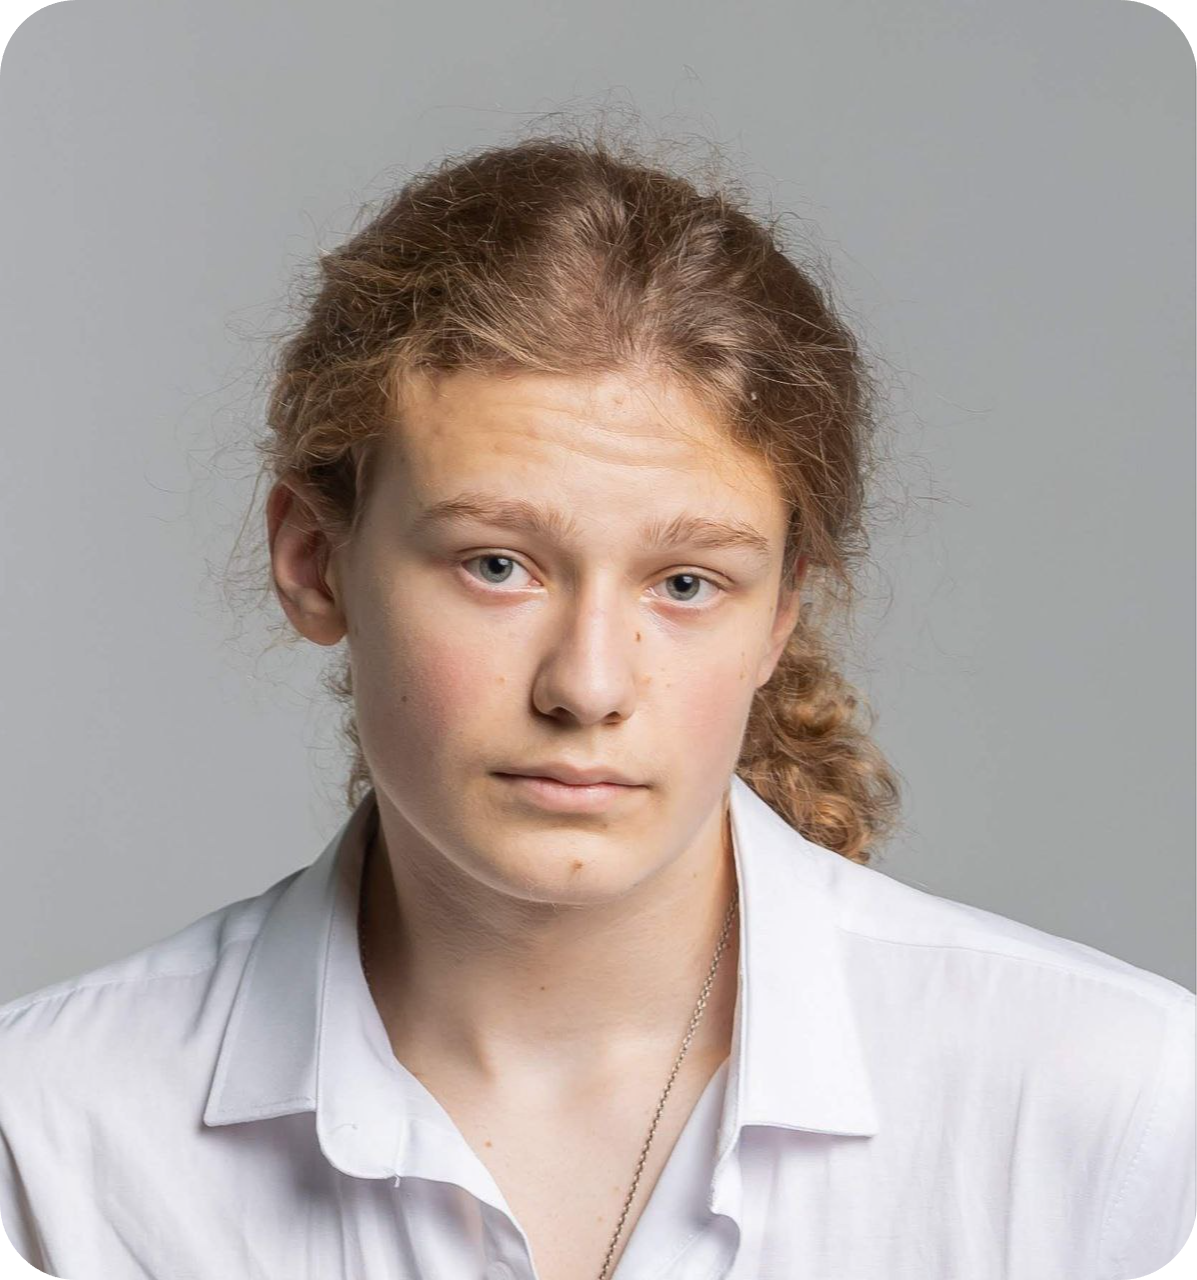
\includegraphics[width=0.270\textwidth]{../images/avatar.png}
    \end{textblock}
  \end{minipage}

  \vspace{-7mm}
  \section{\mysidestyle Обо мне}
  \texttt{Backend}-разработчик и стажёр Яндекса. Развиваю инфраструктуру
  потоковой обработки данных: деплой, \texttt{CI/CD}, динамическую конфигурацию
  и инструменты разработки. Интересуюсь формальной верификацией: изучаю
  \texttt{Software Foundations},
  \href{https://github.com/alchemmist/coq-learning}{доказал 250 теорем на
  \texttt{Coq}}. Увлекаюсь \texttt{Linux} и инструментами разработки.
  \href{https://alchemmist.xyz/teach/individual-education/}{Преподаю} \texttt{Python}, обучил
  более 40 учеников. В прошлом профессиональный
  \href{https://alchemmist.github.io/CV/attachments/sport.pdf}{волейболист}.

  \section{\mysidestyle Опыт работы}\vspace{0.7mm}
  Яндекс --- стажёр-разработчик \hfill {\color{black!50}\textit{май - сентябрь 2026}}\\[1.5mm]
  Пользовательские сессии и логи Поиска, \texttt{HitMaster}:
  \begin{itemize}[leftmargin=4mm, itemsep=0pt, topsep=1pt, parsep=0pt, label=\raisebox{0.2ex}{\scalebox{0.6}{\textbullet}}]
    \item Перевёл деплой двух проектов на \texttt{InfraCtl}: разработал
        генераторы спецификаций на \texttt{Starlark}, разделил монолитные
        стейджи по направлениям обработки данных и встроил их в релизный процесс.
    \item Сделал \texttt{InfraCtl} единым источником данных для генераторов
        конфигов, графов обработки и мониторинга. Вынес общую модель стейджей и
        расчёт ресурсов в переиспользуемую \texttt{Python}-библиотеку.
    \item Подключил \texttt{REX} для обновления геобазы в Поиске. Реализовал
        \texttt{HTTP}-обработчик и потокобезопасную замену геобазы. Сократил
        лаг доставки геобазы до нескольких минут.
    \item Внедрил динамические конфиги через Молнию: \texttt{JSON}-патчи из
        \texttt{Y.Deploy UI} выкатываются за $\sim 1$ минуту. Добавил
        последовательную раскатку и защиту от повторных перебалансировок шардов
        в \texttt{YT}.
    \item Разработал экшен выкатки из \texttt{PR}: выбор контура, компонентов,
        спек и типов артефактов, выборочная сборка и поэтапное продвижение
        релиза. Добавил выкатку спецификаций без пересборки бинарников.
    \item Разработал штатный \texttt{rollback-flow} в \texttt{CI} и автооткат
        по алертам технических метрик. Для выкаток из \texttt{PR}
        реализовал возврат к последнему успешному полному релизу с защитой
        от повторных и устаревших сигналов.
    \item Согласовал и настроил автоформатирование \texttt{Python}, \texttt{C++}
        и \texttt{Starlark}: локальные хуки, \texttt{CI}-линтинг и
        \texttt{commit-suggest} в \texttt{PR}. В рамках этой задачи создал
        \href{https://fq.alchemmist.xyz}{\texttt{format-quorum}} и рассказал про него на
        \href{https://www.youtube.com/watch?v=cz_K6YEIQho}{Хурале}.
  \end{itemize}\vspace{-2mm}
  Стек: \inlinecode{Python}, \inlinecode{C++}, \inlinecode{Starlark},
  \inlinecode{Arcadia CI}, \inlinecode{InfraCtl}, \inlinecode{Y.Deploy},
  \inlinecode{Logbroker}, \inlinecode{Monium}.

  {\let\makelabel\descriptionlabel
    \renewcommand*\descriptionlabel[1]{\hspace\labelsep\normalfont #1}
    \section{\mysidestyle Образование}\vspace{0.7mm}
    \begin{description}[leftmargin=0pt, itemindent=*, itemsep=3pt]
      \item[\href{https://cu.ru}{Центральный университет}.]
        Математика и компьютерные науки, 2028 (2 курс).
        Разработка; траектория \texttt{Computer Science Research}.
      \item[\href{https://lyceum.yandex.ru/}{Лицей Академии Яндекса}.]
        Промышленная разработка, аттестат с отличием.
        Финальный проект --- 100/100.
    \end{description}}

  \section{\mysidestyle Достижения}
  Финалист
  (\href{https://alchemmist.github.io/CV/attachments/russian-chemp-final.pdf}{\texttt{1}})
  \href{https://fsp-russia.ru/}{Чемпионата
  России} по спортивному
  программированию среди 5000 участников. За время чемпионата в
  команде разработали два
  (\href{https://github.com/alchemmist/sport-afisha/}{\texttt{1}},
  \href{https://github.com/alchemmist/sportprog}{\texttt{2}})
  проекта. Технический стек:
  \inlinecode{Kafka}, \inlinecode{React},
  \inlinecode{RabbitMQ (FastStream)},
  \inlinecode{FastAPI},
  \inlinecode{OAuth}.

  \href{https://alchemmist.github.io/CV/attachments/scince-for-life-win.pdf}{Победитель}
  научно-практической конференции
  «\href{https://conf.profil.mos.ru/academ}{Наука для
  жизни}» среди 117 проектов с
  \href{https://github.com/smart-cab/}{проектом умного
  дома}. Технический стек: \inlinecode{Redis},
  \inlinecode{Zigbee2MQTT}, \inlinecode{websockets}, \inlinecode{Go},
  \inlinecode{Python}, \inlinecode{Flask}, \inlinecode{React}.

\end{resume}

\clearpage

\end{document}
